% Font options: 10pm, 11pt, 12pt
% Align headings left instead of center: nocenter
\documentclass[xcolor=x11names,compress]{beamer}\usepackage[]{graphicx}\usepackage[]{color}
%% maxwidth is the original width if it is less than linewidth
%% otherwise use linewidth (to make sure the graphics do not exceed the margin)
\makeatletter
\def\maxwidth{ %
  \ifdim\Gin@nat@width>\linewidth
    \linewidth
  \else
    \Gin@nat@width
  \fi
}
\makeatother

\definecolor{fgcolor}{rgb}{0.345, 0.345, 0.345}
\newcommand{\hlnum}[1]{\textcolor[rgb]{0.686,0.059,0.569}{#1}}%
\newcommand{\hlstr}[1]{\textcolor[rgb]{0.192,0.494,0.8}{#1}}%
\newcommand{\hlcom}[1]{\textcolor[rgb]{0.678,0.584,0.686}{\textit{#1}}}%
\newcommand{\hlopt}[1]{\textcolor[rgb]{0,0,0}{#1}}%
\newcommand{\hlstd}[1]{\textcolor[rgb]{0.345,0.345,0.345}{#1}}%
\newcommand{\hlkwa}[1]{\textcolor[rgb]{0.161,0.373,0.58}{\textbf{#1}}}%
\newcommand{\hlkwb}[1]{\textcolor[rgb]{0.69,0.353,0.396}{#1}}%
\newcommand{\hlkwc}[1]{\textcolor[rgb]{0.333,0.667,0.333}{#1}}%
\newcommand{\hlkwd}[1]{\textcolor[rgb]{0.737,0.353,0.396}{\textbf{#1}}}%
\let\hlipl\hlkwb

\usepackage{framed}
\makeatletter
\newenvironment{kframe}{%
 \def\at@end@of@kframe{}%
 \ifinner\ifhmode%
  \def\at@end@of@kframe{\end{minipage}}%
  \begin{minipage}{\columnwidth}%
 \fi\fi%
 \def\FrameCommand##1{\hskip\@totalleftmargin \hskip-\fboxsep
 \colorbox{shadecolor}{##1}\hskip-\fboxsep
     % There is no \\@totalrightmargin, so:
     \hskip-\linewidth \hskip-\@totalleftmargin \hskip\columnwidth}%
 \MakeFramed {\advance\hsize-\width
   \@totalleftmargin\z@ \linewidth\hsize
   \@setminipage}}%
 {\par\unskip\endMakeFramed%
 \at@end@of@kframe}
\makeatother

\definecolor{shadecolor}{rgb}{.97, .97, .97}
\definecolor{messagecolor}{rgb}{0, 0, 0}
\definecolor{warningcolor}{rgb}{1, 0, 1}
\definecolor{errorcolor}{rgb}{1, 0, 0}
\newenvironment{knitrout}{}{} % an empty environment to be redefined in TeX

\usepackage{alltt}
%\documentclass[xcolor=x11names,compress,handout]{beamer}
\usepackage[]{graphicx}
\usepackage[]{color}
\usepackage{booktabs}
\usepackage{hyperref}
\usepackage{tikz}
\usepackage{multirow}
\usepackage{dcolumn}
\usepackage{bigstrut}
\usepackage{amsmath} 
\usepackage{xcolor,colortbl}
\usepackage{amssymb}
%\newcommand{\done}{\cellcolor{teal}#1}

%% Beamer Layout %%%%%%%%%%%%%%%%%%%%%%%%%%%%%%%%%%
\useoutertheme[subsection=false,shadow]{miniframes}
\useinnertheme{default}
\usefonttheme{serif}
\usepackage{Arev}
\usepackage{pdfpages}

\setbeamerfont{title like}{shape=\scshape}
\setbeamerfont{frametitle}{shape=\scshape, size=\normalsize}

\definecolor{dkblue}{RGB}{0,0,102}

\setbeamercolor*{lower separation line head}{bg=dkblue} 
\setbeamercolor*{normal text}{fg=black,bg=white} 
\setbeamercolor*{alerted text}{fg=red} 
\setbeamercolor*{example text}{fg=black} 
\setbeamercolor*{structure}{fg=black} 
 
\setbeamercolor*{palette tertiary}{fg=black,bg=black!10} 
\setbeamercolor*{palette quaternary}{fg=black,bg=black!10} 

\renewcommand{\(}{\begin{columns}}
\renewcommand{\)}{\end{columns}}
\newcommand{\<}[1]{\begin{column}{#1}}
\renewcommand{\>}{\end{column}}

\setbeamertemplate{navigation symbols}{} 
\setbeamertemplate{footline}[frame number]
\setbeamertemplate{caption}{\raggedright\insertcaption\par}

\setbeamersize{text margin left=5pt,text margin right=5pt}

%%%%%%%%%%%%%%%%%%%%%%%%%%%%%%%%%%%%%%%%%%%%%%%%%%




\title{Making Causal Critiques}
\subtitle{Day 3 - Assessing Causal Evidence}
\author{Jonathan Phillips}
\IfFileExists{upquote.sty}{\usepackage{upquote}}{}
\begin{document}

\frame{\titlepage}

\section{Introduction}

\begin{frame}
\frametitle{Solving the Problem of Causal Inference}
\begin{itemize}
\item We cannot!
\item But we can try and minimize the risks
\item Selecting units that provide appropriate counterfactuals, avoiding:
\begin{itemize}
\item Omitted variable bias
\item Selection Bias
\item Reverse Causation
\end{itemize}
\end{itemize}
\end{frame}

\begin{frame}
\frametitle{Solving the Problem of Causal Inference}
\begin{itemize}
\item Experiments
\begin{itemize}
\item Field Experiments
\item Lab Experiments
\item Survey Experiments
\end{itemize}
\item Quasi-Experiments
\begin{itemize}
\item Instrumental Variables
\item Regresssion Discontinuity
\item Difference-in-DIfferences
\end{itemize}
\end{itemize}
\end{frame}

\begin{frame}
\frametitle{Causal Inference}
\begin{table}[htbp]
  \centering
  \caption{Types of Research Design:}
    \begin{tabular}{|p{3.5cm}|p{3.5cm}|p{3.5cm}|}
    \toprule
          & Researcher controls the treatment assignment & Treatment assignment mechanism likely to create comparable potential outcomes ('Conditional Independence') \\
    \midrule
    Controlled Experiments & Yes   & Yes \\
    \midrule
    Natural Experiments & No    & Yes \\
    \midrule
    Observable Studies & No    & No \\
    \bottomrule
    \end{tabular}%
  \label{tab:addlabel}%
\end{table}%
\end{frame}


\section{Experiments}

\begin{frame} 
\frametitle{Field Experiments}
\begin{itemize}
\item Field experiments provide confidence because treatment assignment is \textbf{controlled by the researcher}
\item But still take place in real-world environments, so they identify (hopefully) meaningful treatment effects
\end{itemize}
\end{frame}

\begin{frame}
\frametitle{Field Experiments}
\begin{itemize}
\item Why does randomization help us achieve causal inference?
\pause
\begin{itemize}
\item A treatment assignment mechanism that \textbf{balances potential outcomes}
\item Every unit has \textbf{exactly the same} probability of treatment
\item If treatment is randomly distributed, \textbf{so are potential outcomes}
\end{itemize}
\item Potential outcomes are - on average - the same for treated and control units
\begin{itemize}
\item No omitted variable bias
\item No self-selection
\item No reverse causation
\end{itemize}
\end{itemize}
\end{frame}

\begin{frame}
\frametitle{Field Experiments}
\begin{itemize}
\item Why does randomization help us achieve causal inference?
\begin{itemize}
\item We want to estimate:
\end{itemize}
\begin{eqnarray}
E(Y_1 - Y_0)
\end{eqnarray}
\pause
\begin{itemize}
\item Our data provides:
\end{itemize}
\begin{eqnarray}
E(Y_1|D=1)\text{ ,  }E(Y_0|D=0)
\end{eqnarray}
\pause
\begin{itemize}
\item With randomization, $Y_1, Y_0 \perp D$:
\pause
\end{itemize}
\begin{eqnarray}
E(Y_1|D=1) &=& E(Y_1) \pause \\
E(Y_0|D=0) &=& E(Y_0) \pause \\
E(Y_1|D=1) - E(Y_0|D=0) &=& E(Y_1) - E(Y_0) \pause \\
&=& E(Y_1 - Y_0)
\end{eqnarray}
\end{itemize}
\end{frame}

\begin{frame}
\frametitle{Field Experiments}
\begin{itemize}
\item But these are just \textbf{expectations} (averages)
\pause
\begin{itemize}
\item \textbf{On average}, potential outcomes will be balanced
\pause
\item More likely in larger samples
\pause
\item We cannot measure potential outcomes
\pause
\item But we can assess balance in \textit{observable} covariates
\pause
\item What if some covariates are imbalanced? %Expected 1/20. Still need to correct as could be real bias.
\end{itemize}
\end{itemize}
\end{frame}

\begin{frame}
\frametitle{Field Experiments}
\begin{itemize}
\item Analysing field experiments
\begin{itemize}
\item Comparison of means: t-test to test significance
\item Regression achieves the same thing
\item $Y_i \sim \alpha + \beta D_i + \epsilon_i$ 
\end{itemize}
\end{itemize}
\end{frame}

\begin{frame}
\frametitle{Field Experiments}
\begin{itemize}
\item Assumptions
\begin{itemize}
\item \textbf{Compliance with randomization} - Treatment was truly random and accepted
\item \textbf{No Spillovers (SUTVA)} - Treatment of one unit doesn't affect potential outcomes of other units
\end{itemize}
\end{itemize}
\end{frame}

\begin{frame}
\frametitle{Field Experiments}
\begin{itemize}
\item Limitations of Field Experiments: 
\pause
\begin{itemize}
\item Small sample sizes still prevent inference
\item Ethics
\item Logistics/Finance
\item Some treatments can't be manipulated (history)
\item Lack of control over treatment content and context - is it informative?
\item Long-term/scale effects/adaptation?
\end{itemize}
\end{itemize}
\end{frame}

\begin{frame}
\frametitle{Field Experiments}
\begin{itemize}
\item Limitations of Field Experiments: \textbf{Internal Validity}
\pause
\begin{itemize}
\item No guarantee of actual balance
\item Unbiased but imprecise; variation still high if lots of other variables also affect Y
\item Hawthorne effect: participants adapt behaviour in experiments
\item Biased measurement if not double-blind
\item \textit{Average} Treatment Effect can be skewed by Outliers
\item Complications of non-compliance, attrition
\end{itemize}
\end{itemize}
\end{frame}

\begin{frame}
\frametitle{Field Experiments}
\begin{itemize}
\item All these complications mean we need lots of assumptions and background knowledge
\item Just as with other methodologies
\end{itemize}
\end{frame}

\begin{frame}
\frametitle{Lab/Survey Experiments}
\begin{itemize}
\item Why lab and survey experiments?
\pause
\begin{itemize}
\item Treatments we cannot administer in reality
\item Outcome measurements that are hard to take in reality
\item Random treatment assignment not permitted in reality
\end{itemize}
\end{itemize}
\end{frame}

\begin{frame}
\frametitle{Lab/Survey Experiments}
\begin{itemize}
\item \textbf{Treatment Assignment}: Same as a Field Experiment
\pause
\item \textbf{Treatment}: Not a manipulation of real world political or economic processes, but establishing controlled 'lab' conditions
\pause
\begin{itemize}
\item The advantage: Control over context helps isolate mechanisms
\item The disadvantage: Can we generalize to the real world from this artificial context?
\end{itemize}
\end{itemize}
\end{frame}

\section{Instrumental Variables}

\begin{frame}
\frametitle{Instrumental Variables}
\begin{itemize}
\item What can we do when the treatment assignment mechanism is not random?
\pause
\item An 'instrument' is a variable which assigns treatment in an 'as-if' random way
\pause
\begin{itemize}
\item Or at least in a way which is 'exogenous' - not related to omitted variables
\item Even if other variables \textbf{also} affect treatment
\end{itemize}
\end{itemize}
\end{frame}

\begin{frame}
\frametitle{Instrumental Variables}
\begin{itemize}
\item We can use the instrument to isolate 'as-if' random variation in treatment, and use that to estimate the effect of treatment on the outcome
\pause
\item NOT the effect of the instrument on the outcome
\end{itemize}
\end{frame}

\begin{frame}
\frametitle{Instrumental Variables}
\begin{itemize}
\item Example Instruments:
\begin{itemize}
\item Rainfall for conflict 
\item Sex-composition for effect of third child
\item Distance from the coast for exposure to slave trade
\end{itemize}
\end{itemize}
\end{frame}

\begin{frame}
\frametitle{Instrumental Variables}
\begin{itemize}
\item Instrumental Variables Assumptions
\begin{itemize}
\item \textbf{Strong First Stage:} The Instrument must \textbf{affect} the treatment
\pause
\item We can test this with a simple regression: $Treatment \sim Instrument$
\pause
\item The instrument should be a significant predictor of treatment
\item Rule-of-thumb: $F-statistic > 10$
\end{itemize}
\end{itemize}
\end{frame}

\begin{frame}
\frametitle{Instrumental Variables}
\begin{itemize}
\item Instrumental Variables Assumptions:
\begin{enumerate}
\item \textbf{No Spillovers (SUTVA)}
\pause
\item \textbf{Strong First Stage (Instrument -> Treatment)}
\pause
\item \textbf{Exclusion Restriction:} The Instrument \textbf{ONLY} affects the outcome through its effect on treatment, and not directly
\pause
\begin{itemize}
\item \textbf{We cannot test or prove this assumption!}
\end{enumerate}
\pause
\end{itemize}
\item Theory and qualitative evidence needed to argue that the instrument is not correlated with any other factors affecting the outcome
\end{itemize}
\end{frame}

\begin{frame}
\frametitle{Instrumental Variables}
\begin{itemize}
\item Instrumental Variables Methodology:
\pause
\begin{enumerate}
\item Use an all-in-one package, eg. \textit{ivreg} in the \textit{AER} package
\begin{itemize}
\item Specify the formula: $Y ~ D | Instrument$
\pause
\end{itemize}
\item Conduct 2-Stage Least Squares: 
\pause
\begin{itemize}
\item Isolate the variation in treatment caused by the instrument: $D \sim Instrument$
\pause
\item Save the predicted values from this regression: $\hat{D} = D \sim Instrument$
\pause
\item Estimate how the predicted values affect the outcome: $Y \sim \hat{D}$
\pause
\item Interpret the coefficient on $\hat{D}$
\end{itemize}
\end{enumerate}
\end{itemize}
\end{frame}

\begin{frame}
\frametitle{Instrumental Variables}
\begin{itemize}
\item IV Interpretation:
\pause
\begin{itemize}
\item Your coefficient is a causal estimate ONLY for units that were actually treated \textbf{because of the instrument}
\pause
\item They don't tell us about the causal effect for other units that never responded to the instrument
\pause
\item We call our causal effect estimate a 'Local Average Treatment Effect' (LATE)
\item 'Local' to the units whose treatment status actually changed
\end{itemize}
\end{itemize}
\end{frame}



\section{Regression Discontinuities}

\begin{frame}
\frametitle{Regression Discontinuities}
\begin{itemize}
\item As always, we need some 'as-if' random variation in assignment to treatment to get plausible counterfactuals
\pause
\item Regression discontinuities take advantage of social rules that \textbf{treat similar people differently}
\pause
\item Specifically, similar people with slightly different 'scores' are assigned to treatment/control
\end{itemize}
\end{frame}

\begin{frame}
\frametitle{Regression Discontinuities}
\begin{center}
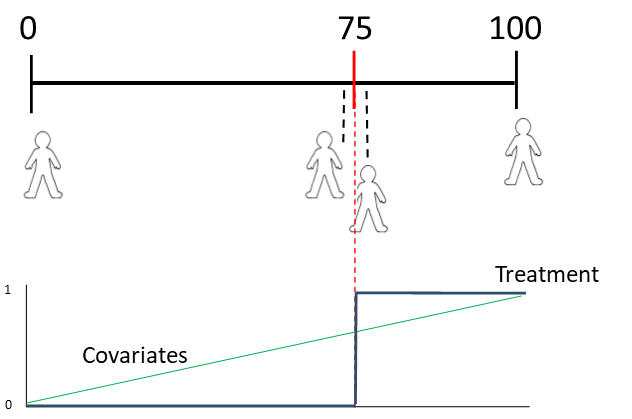
\includegraphics[scale=0.45]{Scale.png}
\end{center}
\end{frame}

\begin{frame}
\begin{itemize}
\item Regression Discontinuity
\begin{itemize}
\item Treatment assignment is 'as-if' random only \textbf{really close to the threshold}
\pause
\[
D_i=
\begin{cases}
1 & \text{if }x_i \geq \bar{x} \\
0 & \text{if }x_i < \bar{x}
\end{cases}
\]
\pause
\item For units just above and below the threshold:
\begin{itemize}
\item Their covariates are almost the same
\item Their potential outcomes are (on average) almost the same
\item They are plausible counterfactuals for each other
\end{itemize}
\pause
\item So we can compare them directly
\end{itemize}
\end{itemize}
\end{frame}

\begin{frame}
\begin{itemize}
\item Example thresholds:
\begin{itemize}
\item Exam cutoffs
\item Age cutoffs
\item Policy eligibility rules
\item Close elections
\item Adminsitrative boundaries
\end{itemize}
\end{itemize}
\end{frame}

\begin{frame}
\begin{itemize}
\item Regresssion Discontinuity Variables:
\begin{itemize}
\item \textbf{Running Variable, $x_i$:} The \textit{continuous} variable to which the threshold/cutoff is applied, eg. exam score
\pause
\item \textbf{Treatment, $D_i$:} Binary 0/1 depending on whether the running variable is above or below the threshold ($x_i>=\bar{x}$)
\pause
\item \textbf{Outcome, $Y_i$:} Any subsequent outcome you have measured
\end{itemize}
\end{itemize}
\end{frame}

\begin{frame}
\begin{itemize}
\item Regression Discontinuity Assumptions:
\begin{enumerate}
\item No spillovers (SUTVA)
\pause
\item Potential outcomes vary continuously (are independent of treatment) at the threshold
\pause
\item Units cannot precisely 'manipulate' their score and sort either side of the threshold
\pause
\item The threshold is not chosen strategically
\pause
\item No compound treatments
\end{enumerate}
\end{itemize}
\end{frame}

\begin{frame}
\begin{itemize}
\item The threshold is more likely to be exogenous if:
\pause
\begin{itemize}
\item Units are not aware of the threshold
\pause
\item The threshold is decided after units make choices
\pause
\item The running variable is hard to manipulate precisely
\pause
\end{itemize}
\item We need qualitative evidence to support these assumptions
\end{itemize}
\end{frame}

\begin{frame}
\begin{itemize}
\item We can check for sorting with a density test
\item If units are bunched just above the threshold, this suggests manipulation
\end{itemize}

\begin{center}
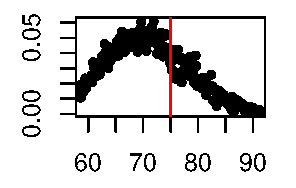
\includegraphics[scale=2]{figure/Density-2.pdf}
\end{center}
\end{frame}

\begin{frame}
\begin{itemize}
\item \textbf{'Parametric' regression discontinuity:} Uses all the data and estimates:
$$Y_i = \alpha + \beta_1 Running\_Variable_i + \beta_2 Treatment_i + \epsilon_i$$
\pause
\begin{itemize}
\item We just control for the 'smooth' variation in the running variable and estimate the 'jump' impact of treatment with a binary variable (dummy)
\pause
\item We may need to make the running variable non-linear
\end{itemize}
\end{itemize}
\end{frame}


\begin{frame}
\frametitle{Raw Data}
\begin{center}
\begin{knitrout}
\definecolor{shadecolor}{rgb}{0.969, 0.969, 0.969}\color{fgcolor}
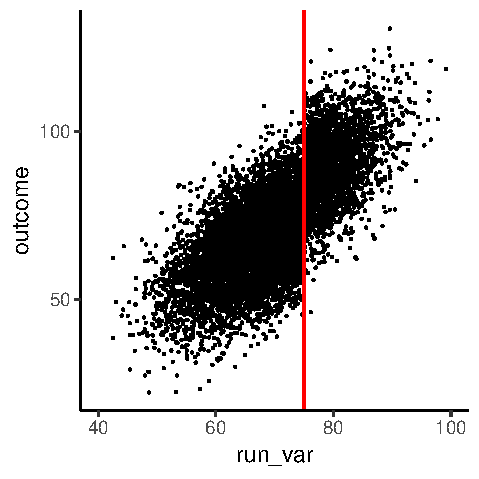
\includegraphics[width=\maxwidth]{figure/chart1-1} 

\end{knitrout}
\end{center}
\end{frame}

\begin{frame}
\frametitle{'Binned' Data}
\begin{center}
\begin{knitrout}
\definecolor{shadecolor}{rgb}{0.969, 0.969, 0.969}\color{fgcolor}
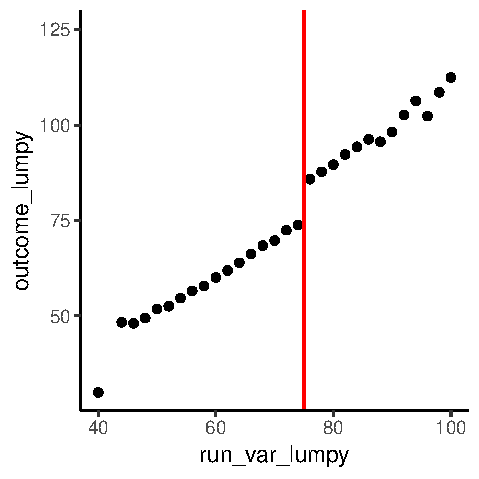
\includegraphics[width=\maxwidth]{figure/chart2-1} 

\end{knitrout}
\end{center}
\end{frame}

\begin{frame}
\frametitle{Difference-in-Means}
\begin{center}
\begin{knitrout}
\definecolor{shadecolor}{rgb}{0.969, 0.969, 0.969}\color{fgcolor}
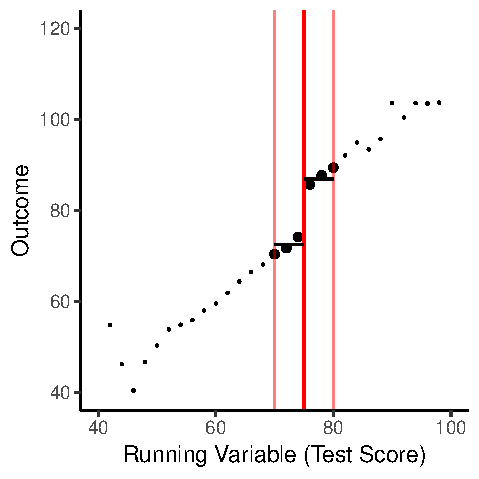
\includegraphics[width=\maxwidth]{figure/chart3-1} 

\end{knitrout}
\end{center}
\end{frame}

\begin{frame}
\frametitle{Parametric Regression - Linear}
\begin{center}
\begin{knitrout}
\definecolor{shadecolor}{rgb}{0.969, 0.969, 0.969}\color{fgcolor}
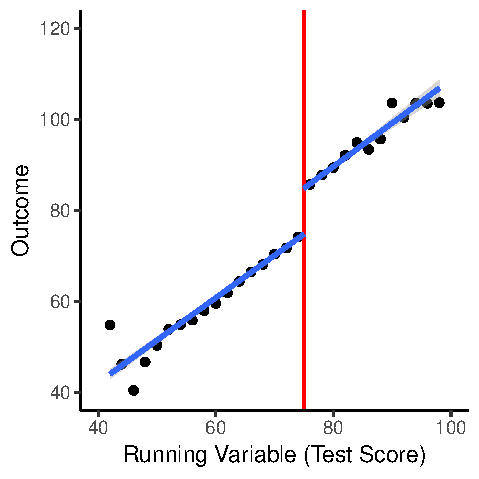
\includegraphics[width=\maxwidth]{figure/chart4-1} 

\end{knitrout}
\end{center}
\end{frame}

\begin{frame}
\frametitle{Parametric Regression - Non-linear}
\begin{center}
\begin{knitrout}
\definecolor{shadecolor}{rgb}{0.969, 0.969, 0.969}\color{fgcolor}
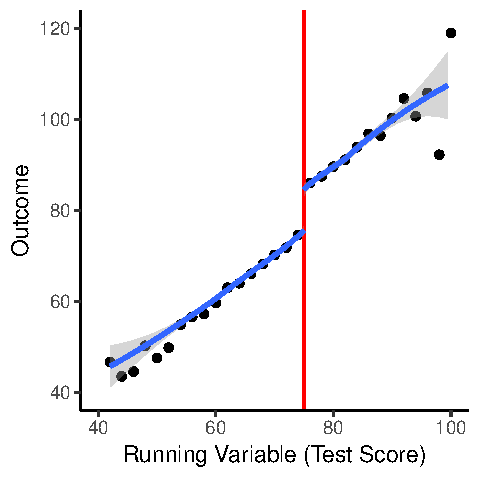
\includegraphics[width=\maxwidth]{figure/chart5-1} 

\end{knitrout}
\end{center}
\end{frame}

\begin{frame}
\begin{itemize}
\item Why does RD estimate a \textbf{Local} Average Treatment Effect?
\pause
\begin{itemize}
\item Treatment assignment is only random at the threshold
\pause
\item Our estimates only apply to units close to the threshold
\pause
\item Units far from the threshold are very different for a reason, and causal effects are likely to be different
\end{itemize}
\end{itemize}
\end{frame}


\begin{frame}
\begin{itemize}
\item Limitations:
\begin{itemize}
\item Risk of sorting/manipulation
\pause
\item Lots of alternative specifications so no single simple test
\pause
\item Opportunistic regression discontinuities may not identify a useful causal effect or for a relevant group
\pause
\end{itemize}
\end{itemize}
\end{frame}

\begin{frame}
\begin{itemize}
\item Close elections are one type of regression discontinuity in which political office is 'as-if' randomized
\pause
\item Particularly useful for understanding the effects of political power
\pause
\begin{itemize}
\item \textbf{Running Variable: }Margin of victory
\item \textbf{Treatment: }Winning a close election
\item \textbf{Control: }Losing a close election
\item \textbf{Outcome: }Anything that happens later...
\end{itemize}
\end{itemize}
\end{frame}

\begin{frame}
\begin{itemize}
\item How much faith should we have in 'close election' regression discontinuities?
\pause
\item Eggers et al (2013):
\pause
\begin{itemize}
\item US House of Representatives elections show sorting in very close elections (<1\%)
\pause
\item Politicians (incumbents, the wealthy) can control whether they win, even when it's a tight race
\pause
\item They have extremely detailed information to predict vote results
\pause
\item So potential outcomes are not balanced
\pause
\item But no other case (9 countries) has this problem
\end{itemize}
\end{itemize}
\end{frame}



\section{Difference-in-Differences}

\begin{frame}
\frametitle{Difference-in-Differences}
\begin{itemize}
\item Some treatments happen at a specific point in time
\begin{itemize}
\item Can't we compare the same unit before and after treatment?
\pause
\item Surely this limits the number of omitted variables - Chile today is very similar to Chile tomorrow
\end{itemize}
\item But No!
\begin{itemize}
\item Other factors influencing the outcome might also have changed between our measurements (eg. any news event!)
\item Eg. a worldwide recession
\end{itemize}
\end{itemize}
\end{frame}

\begin{frame}
\frametitle{Difference-in-Differences}
\begin{itemize}
\item But what if we combine the time-series and cross-section variation?
\pause
\item We can keep lots of variables fixed if we compare the same unit before and after treatment
\pause
\item We can measure how much other factors changed over time if we have units that were not exposed to treatment
\pause
\item There is nothing 'random' here, but we are more easily able to limit the risk of omitted variables
\end{itemize}
\end{frame}

\begin{frame}
\frametitle{Difference-in-Differences}
\begin{knitrout}
\definecolor{shadecolor}{rgb}{0.969, 0.969, 0.969}\color{fgcolor}
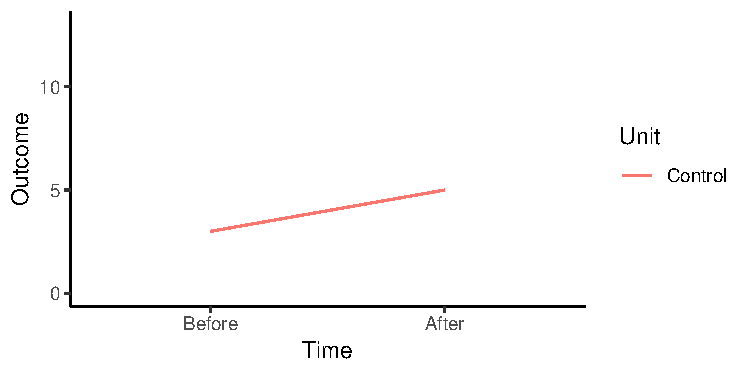
\includegraphics[width=\maxwidth]{figure/DinD_chart1-1} 

\end{knitrout}
\end{frame}


\begin{frame}
\frametitle{Difference-in-Differences}
\begin{knitrout}
\definecolor{shadecolor}{rgb}{0.969, 0.969, 0.969}\color{fgcolor}
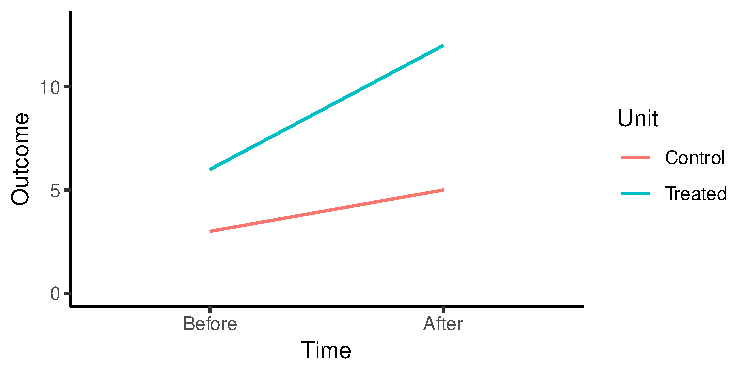
\includegraphics[width=\maxwidth]{figure/DinD_chart1b-1} 

\end{knitrout}
\end{frame}

\begin{frame}
\frametitle{Difference-in-Differences}
\begin{knitrout}
\definecolor{shadecolor}{rgb}{0.969, 0.969, 0.969}\color{fgcolor}
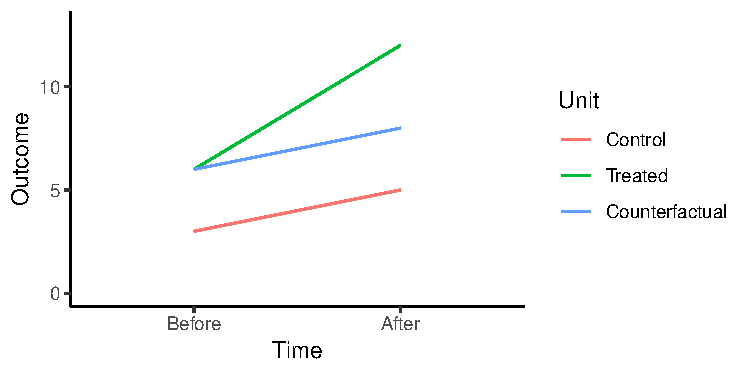
\includegraphics[width=\maxwidth]{figure/DinD_chart1c-1} 

\end{knitrout}
\end{frame}

\begin{frame}
\frametitle{Difference-in-Differences}
\begin{itemize}
\item Example: How has Brexit affected the UK's growth rate?
\pause
\begin{itemize}
\item Comparing with European growth rates is biased - UK growth is influenced by oil, different labour laws etc.
\pause
\item Comparing before and after Brexit is biased - the world economy improved around the same time as Brexit (coincidentally)
\pause
\item But compare how European growth changes (-0.05\%) and UK growth changed (-0.4\%)
\pause
\item The net effect of Brexit is -0.35\%
\pause
\item That's two differences
\begin{itemize}
\item \textbf{Difference 1:} Between before and after (over time)
\item \textbf{Difference 2:} Between treated and control units
\pause
\end{itemize}
\end{itemize}
\end{itemize}
\end{frame}

\begin{frame}
\frametitle{Difference-in-Differences}
\begin{center}
\includegraphics[scale=0.3]{figure/UK_growth.png}
\end{center}
\end{frame}

\begin{frame}
\frametitle{Difference-in-Differences}
\begin{itemize}
\item We're now comparing \textit{changes} (differences), not \textit{levels} of the outcome
\begin{itemize}
\item Most omitted variables affect 'levels', so this makes our counterfactuals more plausible
\begin{itemize}
\item Eg. different laws affect growth rates, not the change in growth over time
\end{itemize}
\item And crucially, we can remove omitted variables even for \textit{unobserved} confounders
\end{itemize}
\end{itemize}
\end{frame}

\begin{frame}
\frametitle{Difference-in-Differences}
\begin{itemize}
\item Difference-in-differences only removes \textbf{time-invariant ('levels') confounders}
\pause
\begin{itemize}
\item Most omitted variables affect 'levels', so this makes our counterfactuals more plausible
\pause
\item Eg. different laws affect growth rates, not the change in growth over time
\pause
\end{itemize}
\item We still need to \textit{make the assumption or argument} that there are \textbf{no time-varying confounders}
\pause
\item Factors that affect the \textbf{trend} in the outcome \textit{differentially} in treated and control units
\pause
\item Eg. Even before Brexit, the UK had falling growth while growth in the eurozone was improving
\end{itemize}
\end{frame}


\begin{frame}
\frametitle{Difference-in-Differences}
\begin{itemize}
\item Estimating Difference-in-Differences
\pause
\item Time (Before and after) and treatment status (treated and control) are just variables in our data
\pause
\item We know how to do a regression for the effect of treatment status on the outcome
\end{itemize}
$$ Y_{it} = \alpha + \gamma D_i$$
\pause
\begin{itemize}
\item The difference-in-differences estimate is just the \textit{interaction} of time and treatment status
\end{itemize}
$$ Y_{it} = \alpha + \gamma D_i + \delta T_t + \beta D_i * T_t $$
\begin{itemize}
\item $\beta$ is our causal effect estimate
\end{itemize}
\end{frame}

\begin{frame}
\frametitle{Difference-in-Differences}
\begin{itemize}
\item Assumptions Required:
\begin{enumerate}
\item No time-varying confounders (Parallel trends)
\item Well-defined treatment (many things changed at the same time!)
\begin{itemize}
\item Eg. The UK also announced new rules to regulate the
banking sector on the same day as Brexit
\end{itemize}
\item Groups are stable (eg. no migration due to treatment)
\end{enumerate}
\end{itemize}
\end{frame}

\begin{frame}
\frametitle{Difference-in-Differences}
\begin{itemize}
\item How do we know if there are time-varying confounders?
\pause
\item We really want the outcome for the treated group to have the same trend as the control group
\pause
\begin{itemize}
\item So any difference in trend is only due to treatment
\pause
\end{itemize}
\item One test of this is to check if \textbf{pre-treatment trends are parallel}
\pause
\item Then our counterfactual makes sense
\end{itemize}
\end{frame}

\begin{frame}
\frametitle{Difference-in-Differences}
\begin{knitrout}
\definecolor{shadecolor}{rgb}{0.969, 0.969, 0.969}\color{fgcolor}
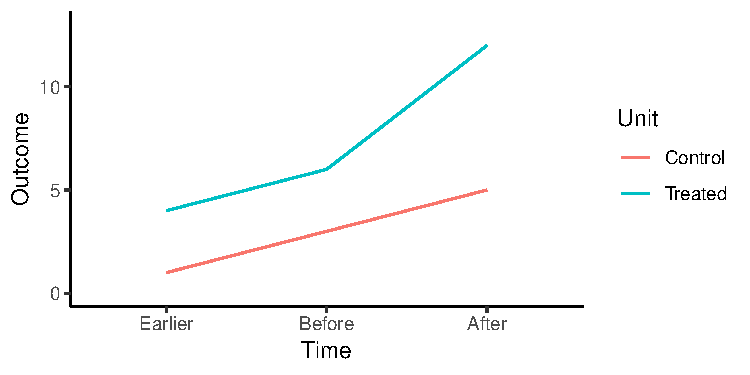
\includegraphics[width=\maxwidth]{figure/DinD_chart6-1} 

\end{knitrout}
\end{frame}

\begin{frame}
\frametitle{Difference-in-Differences}
\begin{knitrout}
\definecolor{shadecolor}{rgb}{0.969, 0.969, 0.969}\color{fgcolor}
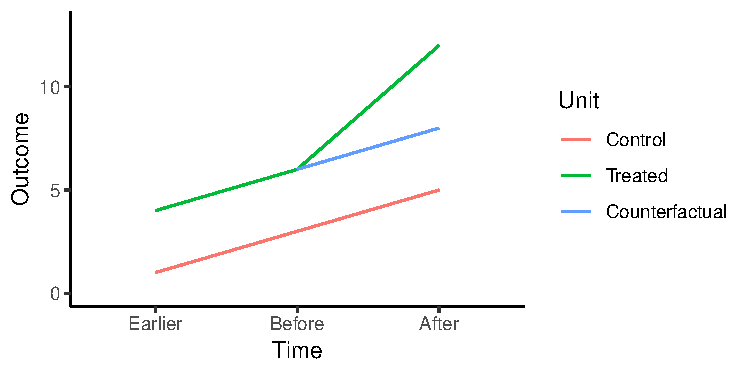
\includegraphics[width=\maxwidth]{figure/DinD_chart7-1} 

\end{knitrout}
\end{frame}

\begin{frame}
\frametitle{Difference-in-Differences}
\begin{itemize}
\item No spillovers (SUTVA)
\pause
\item Parallel trends (no time-varying confounders) is a difficult assumption
\pause
\item Selection into treatment is usually not just due to mostly 'fixed' variables (eg. gender) but due to 'time-varying' variables (eg. income, employment etc.)
\pause
\item Eg. training program participants' income has usually fallen a lot in the past few months
\end{itemize}
\end{frame}

\begin{frame}
\frametitle{Assumptions}
\footnotesize
\begin{table}[htbp]
  \centering
  \caption{Causal Methodology Assumptions}
    \begin{tabular}{|p{3cm}|p{6cm}|}
    \hline
    \textbf{Research Design} & \textbf{Assumptions required for valid causal inference} \bigstrut\\
    \hline
    Field Experiments & No spillovers, Randomization implemented correctly, Randomization complied with, No Hawthorne Effects \bigstrut\\
    \hline
    Lab/Survey Experiments & No spillovers, Randomization implemented correctly, Randomization complied with, No Hawthorne Effects \bigstrut\\
    \hline
    Instrumental Variables & No Spillovers, First stage predicts treatment, Exclusion restriction \bigstrut\\
    \hline
    Regression Discontinuities & No Spillovers, Continuity (balance) of covariates, No precise manipulation, No strategic threshold, No compounding discontinuities \bigstrut\\
    \hline
    Difference-in-Differences & No Spillovers, No time-varying confounders (parallel trends), Well-defined treatment, Stable groups \bigstrut\\
    \hline
    \end{tabular}%
  \label{tab:addlabel}%
\end{table}%
\normalsize
\end{frame}



\end{document}
 
 % Add summary table of assumptions at end, or better: Suggested points of vulnerability to critique
 
 
